\documentclass{article}
\usepackage{amsmath}
\usepackage{hyperref}
\usepackage{graphicx}
%\usepackage[hidelinks]{hyperref}
\textwidth 6.6in \addtolength{\oddsidemargin}{-2.2cm} \textheight 9in \addtolength{\topmargin}{-1in} \setlength{\parindent}{0pt} \setlength{\parskip}{0.5cm} \topskip 0.0in \everymath{\displaystyle} \pagestyle{empty}
\title{Machine Learning (CS 771) \\ Classifying Heart Sounds Challenge}
\author{Rishabh Nigam(10598) \\ Rajesh Shubhankar (13111048) \\ Richa Sharma (13111049) \\ Atulya Shivam Shree(10172) \\ Group 12}
\date{Nov 15}

\hypersetup{
    colorlinks=false,
    pdfborder={0 0 0},
}
\begin{document}
\maketitle

\section{Problem statement and challenges}
There are 2 challenges as follows. \\ \\
\textbf{CHALLENGE 1 - Heart Sound Segmentation} 

The first challenge is to produce a method that can locate $S_1$(lub) and $S_2$(dub) sounds within audio data, segmenting the Normal audio files in both datasets. We need to use the segmented dataset which provides location of $S_1$ and $S_2$ sounds to identify and locate the $S_1$ and $S_2$ sounds of all the heartbeats in the unlabeled group.

\textbf{CHALLENGE 2 - Heart Sound Classification}

The task is to produce a method that can classify real heart audio (also known as “beat classification”) into one of four categories for Dataset A: 
\begin{enumerate}
\item Normal
\item Murmur
\item Extra Heart Sound
\item Artifact
\end{enumerate}
and three classes for Dataset B:
\begin{enumerate}
\item Normal
\item Murmur
\item Extrasystole
\end{enumerate}

\section{Literature review about the problem (Past approaches for similar problems)}

Some of the common things in each of the earlier methods we came across were
\begin{itemize}
\item  Filtering low frequency data, this is based on the premise that the heart sound is low frequency and most energy is concentrated in the region below 195 Hz.
\item  Using Hilbert Transformation and then Calculating Shannon energy. This comes from some of the earlier work done in 1997 by $Liang^{[1]}$.
\item Using some kind of smoothing on the curve and then using the derivative change to find all possible points of local maxima and minima.
\item This is generally followed by fitting nearby maxima/minima by a parabola, and replacing all the nearby points with the peak of the parabola.
\item After we get the peaks, then classification of lub dub sound is based on the length of the diastolic and systolic period. In general we use the fact that in normal sound the pattern is always ... lub dub lub dub ... and the fact that diastolic period was longer than systolic period.
\end{itemize}
Classification of sounds is generally based on some kind of decision tree with parameters being related to the number of peaks, mean and variance of the systolic/diastolic period length. There has not been a concrete approach in any of the methods we came across, so this area is much more open for experimentation as compared to the classification of lub dub points, where the literature is quite concrete.

\section{Dataset}
Dataset is available in .wav and .aif format. We have used data from .wav format. Dataset A contains data at 44100 frames per second, Dataset B at 4000 frames per second. For training, segmentation data (i.e. the actual position of lub and dub sounds) is provided in a csv for 21 and 90 files for dataset A and B respectively.\\
\graphicspath{ {Images/} }

\section{Step involved in Challenge 1}

\subsection{Decimation of data}
Decimate the signal by a factor of 20 for dataset A and for 2 for dataset B. This brings down the frequency close to 2000 for both the datasets. Normalize the signal to (-1,1).\\


\subsection{Calculation of Shannon Energy}
Shannon energy is calculated for continuous 0.02 seconds with an overlap 0.01 second. This is based on the paper by Liang. \\
Shannon energy is defined as $-\frac{1}{N} * \sum_{i=0}^{N-1}{x^2(i) * ln[x^2(i)]}$

\subsection{Smoothening of Shannon Energy}
The Shannon energy obtained in the above step is smoothened using a triangular smooth. Below we show all the results obtained after each step.
\begin{center}
\begin{figure}
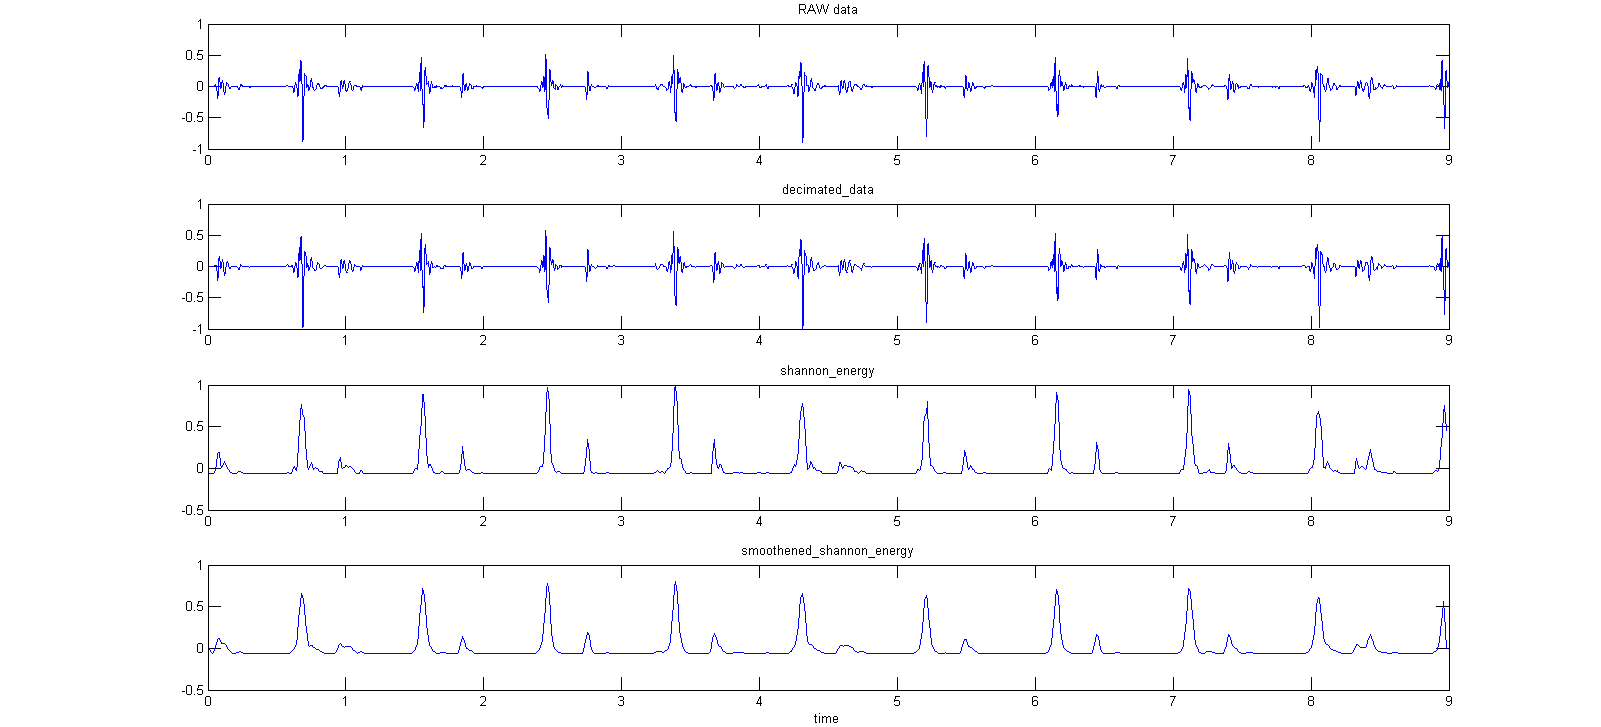
\includegraphics[width=500pt, height=300pt]{ATraining_8_Steps1to4.png}
\caption{Steps 1-4 of Pre-Processing}
\end{figure}
\end{center}
\newpage
\subsection{Calculation of $S_1$ Peaks}
\subsubsection{Getting all Peaks above a threshold}
For peak detection we start of with a heuristic value of threshold and extract all values above it. These values are then passed on to the $S_1$ detection algorithm. 

\subsubsection{Getting $S_1$ Peaks}
In this we start with the assumption the $S_1$ peaks have higher energy. Fist step is to pick the peak with the maximum energy. 

\begin{figure}
\begin{center}
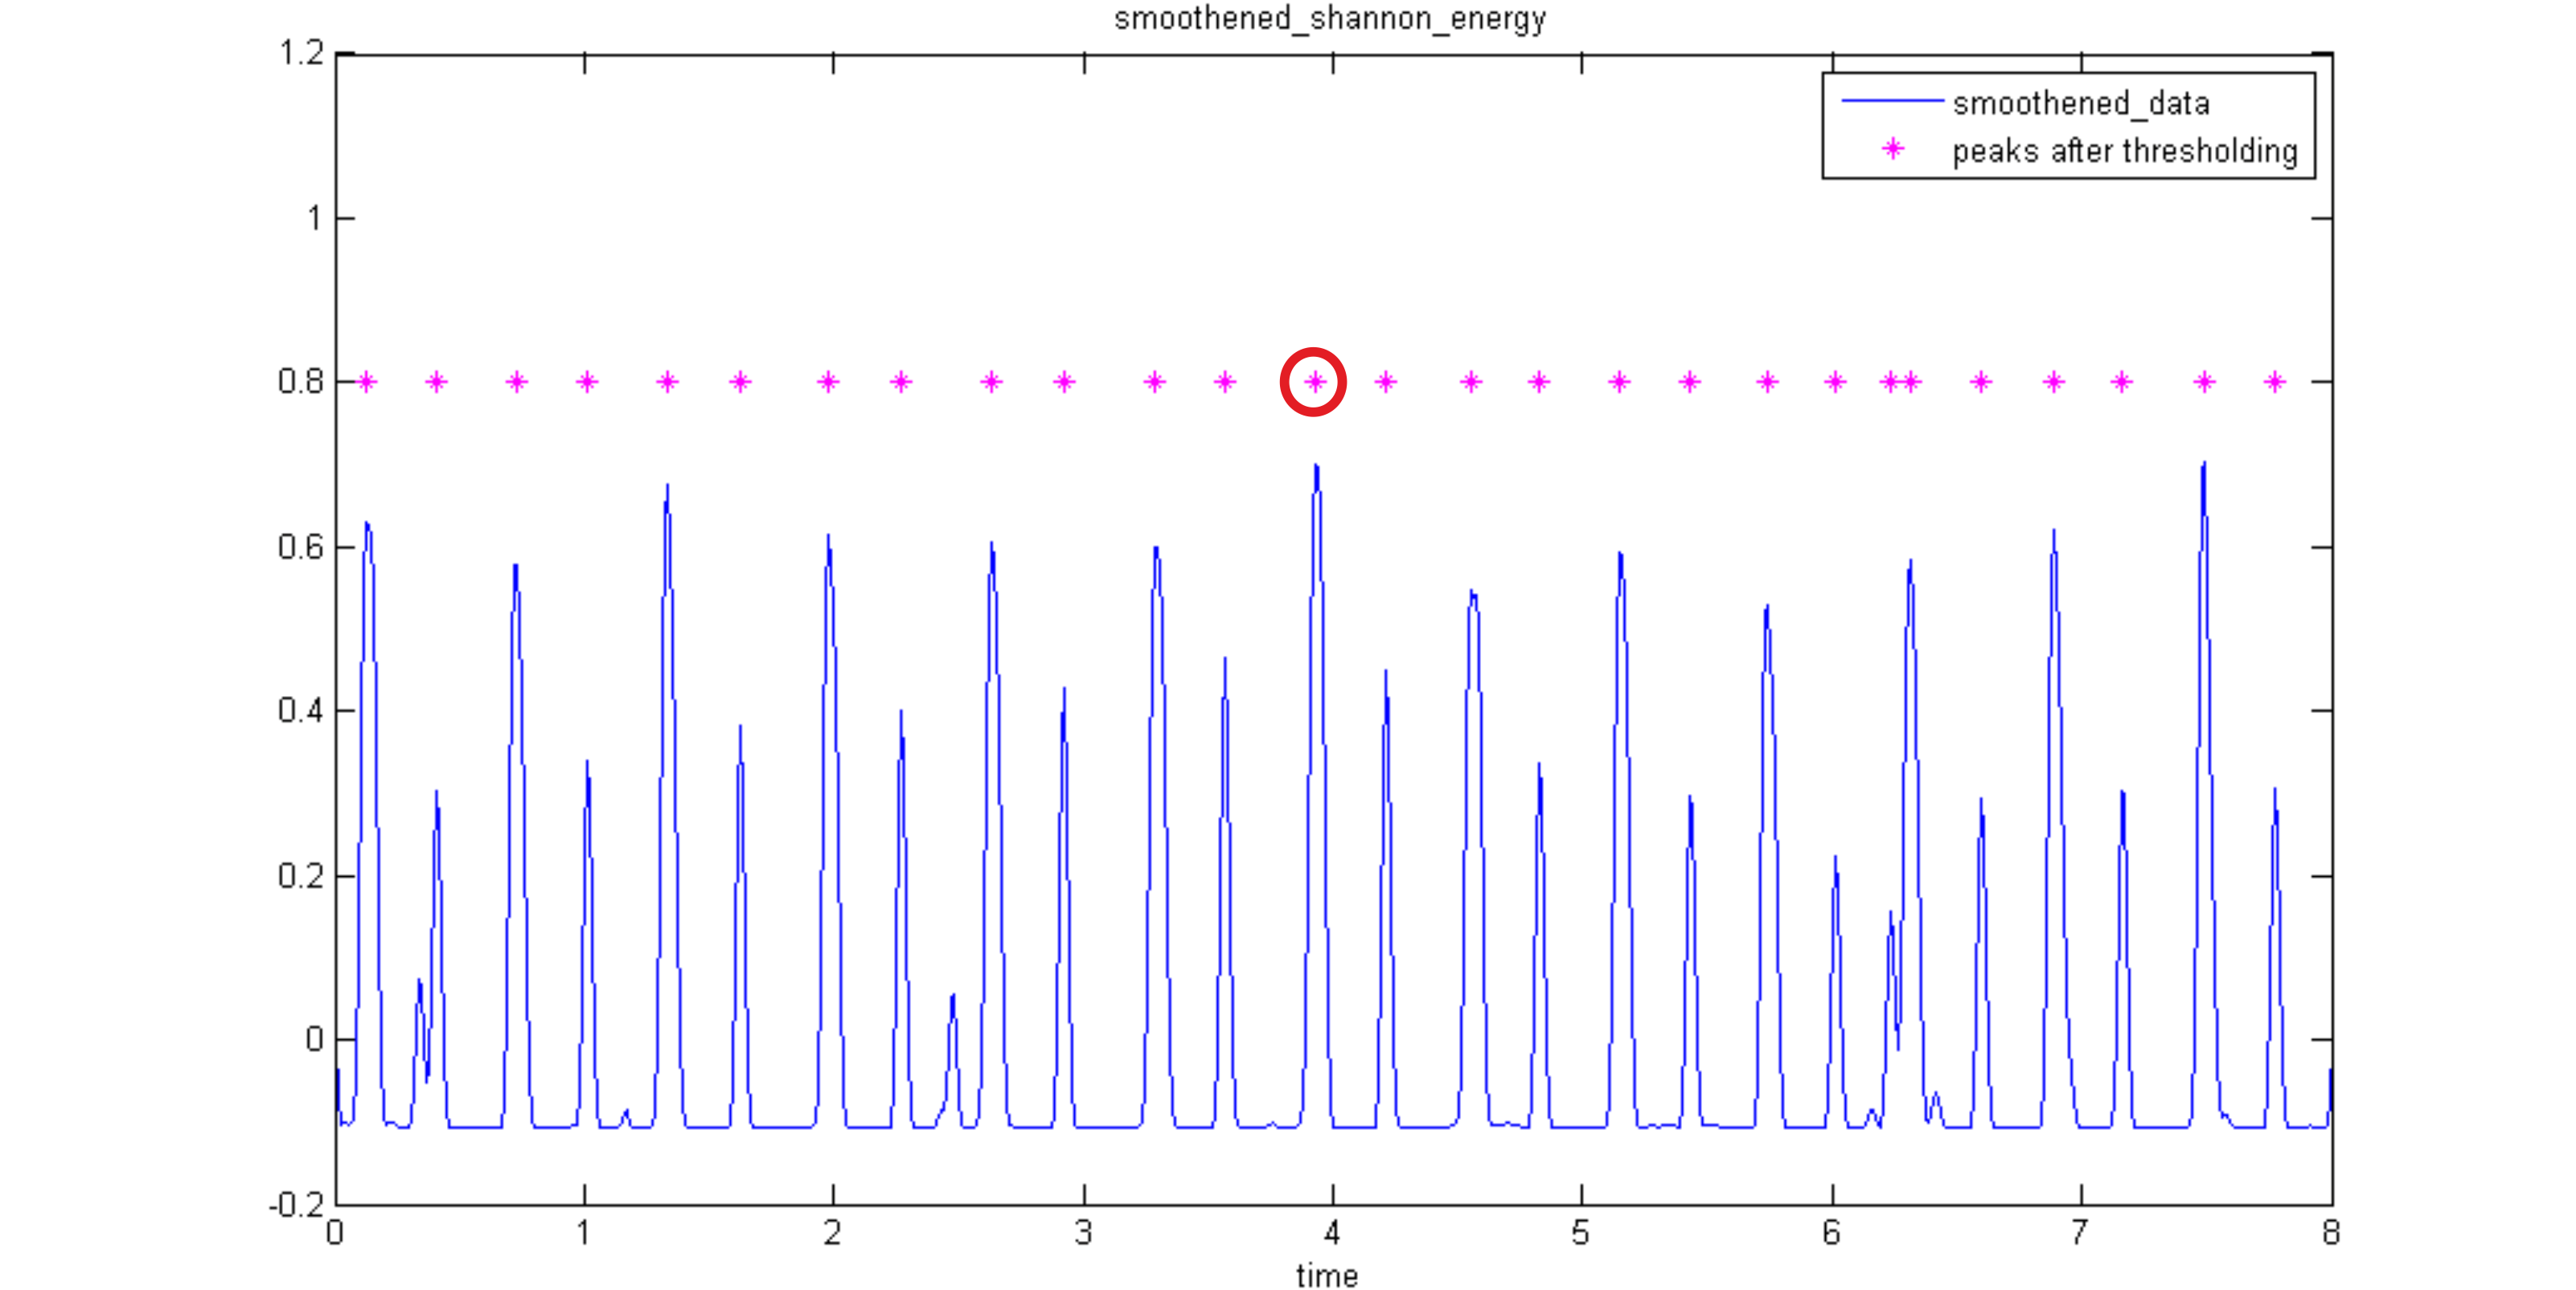
\includegraphics[width=400pt, height=200pt]{detect_max_peak.png}\\
\caption{detecting the peak with the maximum amplitude}
\end{center}
\end{figure}

Then we look for peaks that are one time period away from the maximum peak. These are further added to our list of $S_1$ Peaks. With three new $S_1$ Peaks the time period is updated to get a better estimate of its value. The algorithm then again runs over the instance with a new value of initial time period estimate. In this way the time period is varied from 0.4 to 1.2 seconds covering a heart-beat range of 48 per minute to 150 per minute. Since the time period is updated after finding every $S_1$ peak hence for any instance we are able to get a frequency locked value of the time period in case there are a number of peaks in the signal. Since this can be disturbed by extra peaks in the data we look for that set frequency in the dataset for which the $S_1$ peaks thus obtained have the maximum value of Shannon energy. In this way we get all the $S_1$ peaks and also a set value of the frequency.\\

\begin{figure}
\begin{center}
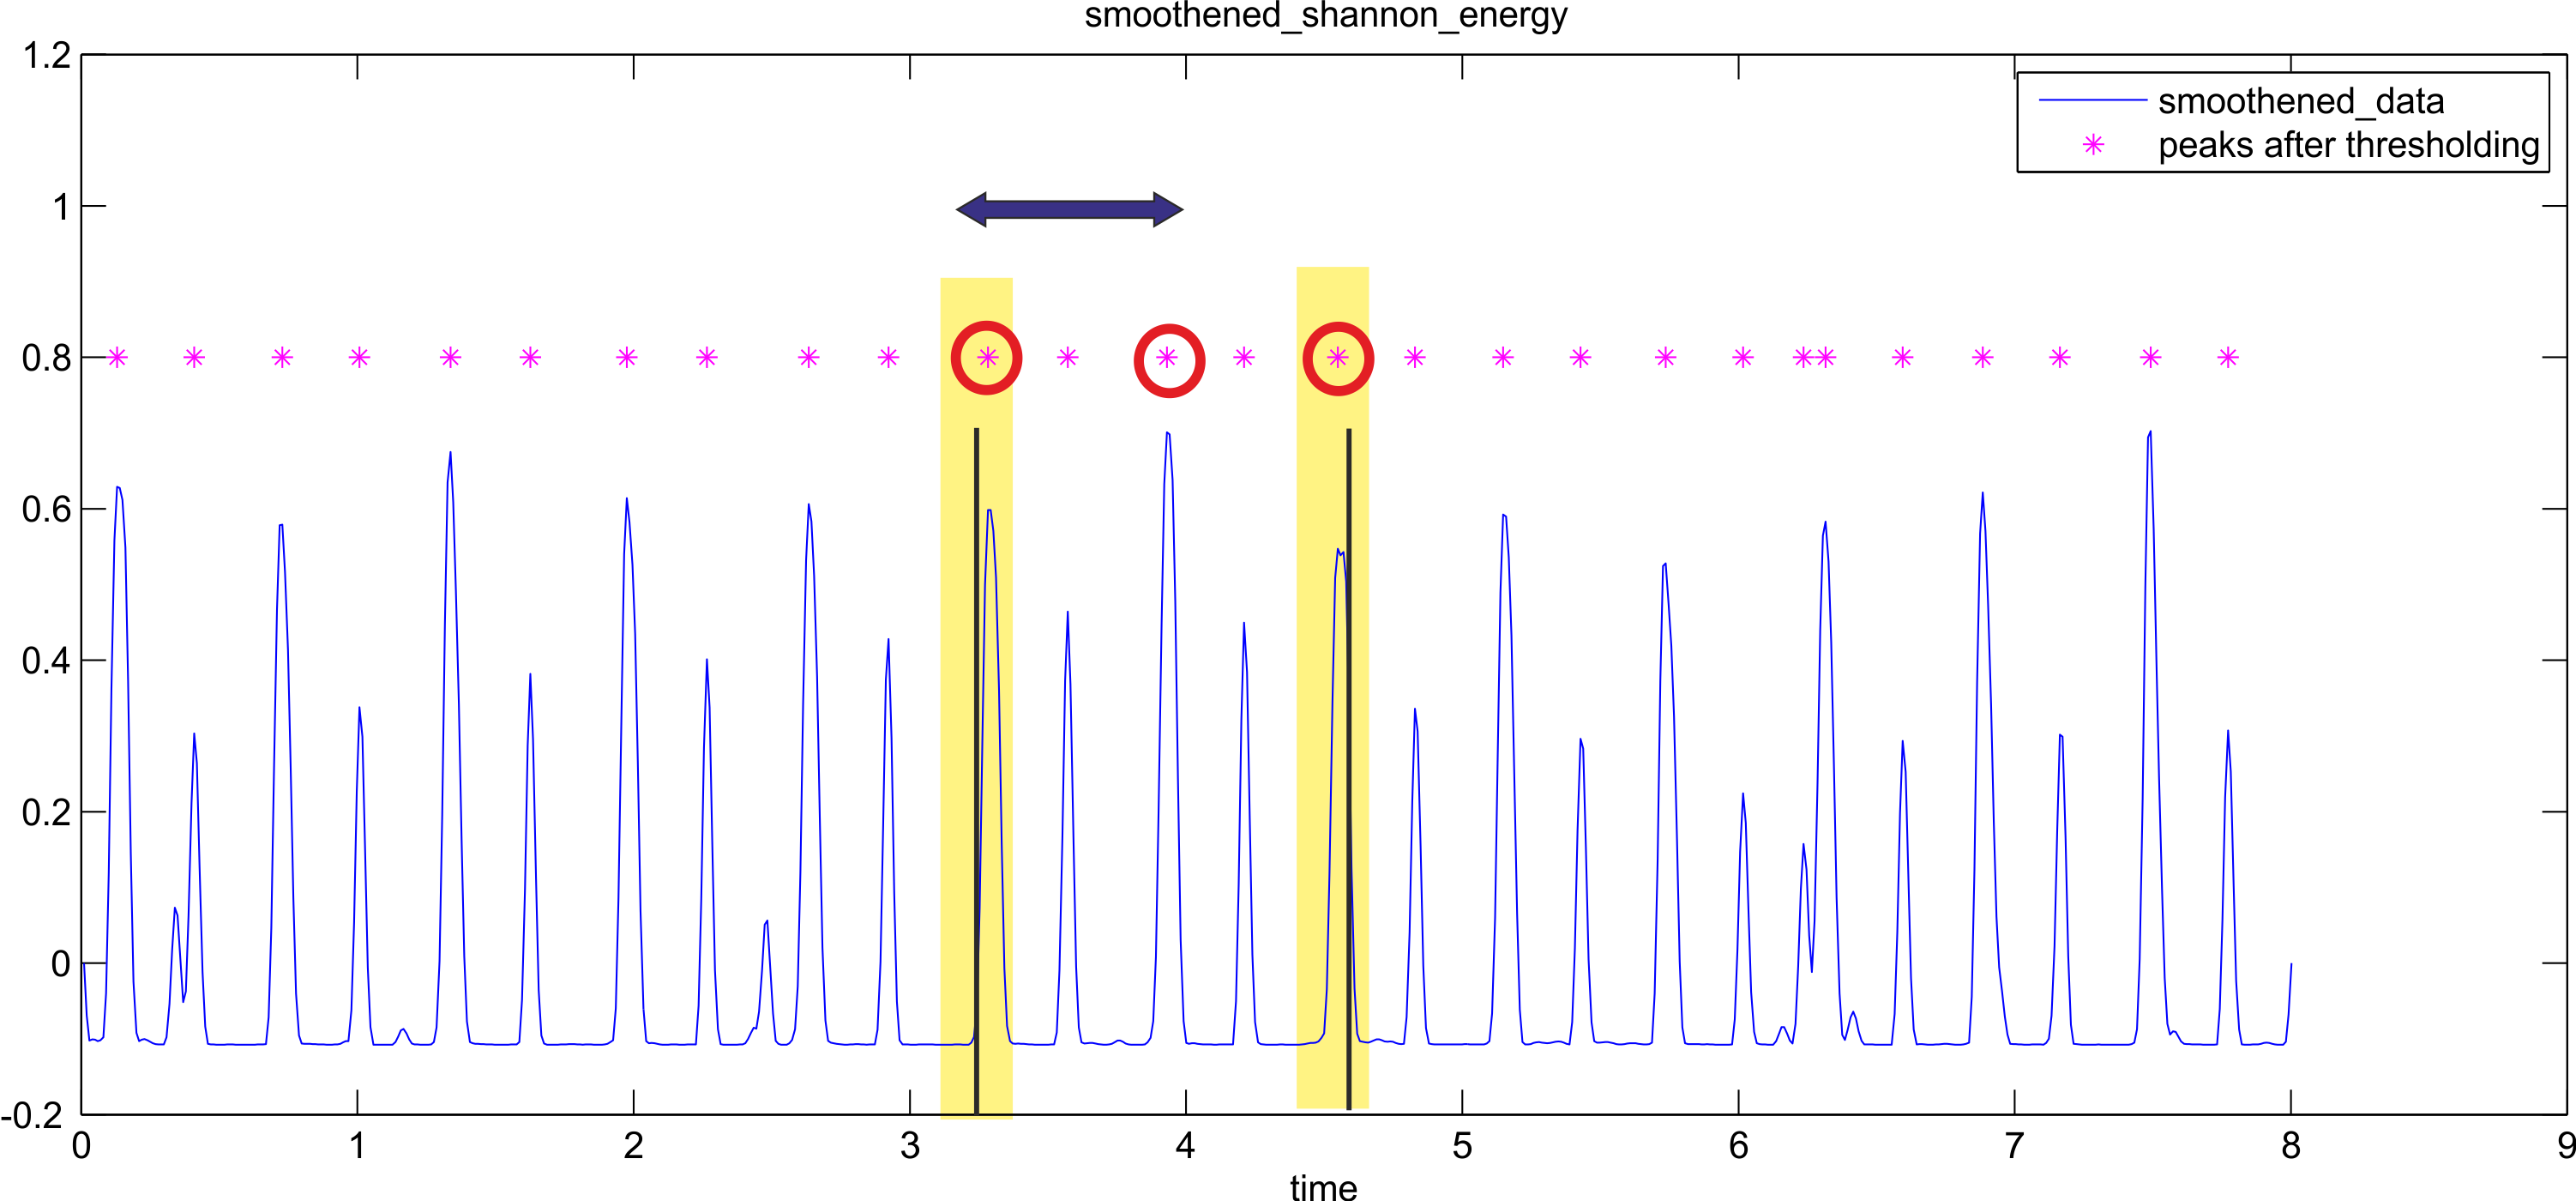
\includegraphics[width=400pt, height=200pt]{detect_other.png}
\caption{Searching for the consecutive $S_1$Peaks with an initial estimate of the time period}
\end{center}
\end{figure}


 

\subsubsection{Getting $S_2$ Peaks}
In the next step the goal is to find the $S_2$ peaks in the signal. For this we have used the thresholded peaks after step1 and the $S_1$ peaks obtained after step 2. We search for peaks in the thresholded that are near midway of two $S_1$ peaks in the thresholded peaks. In case no such peak exists between two $S_1$ peaks the threshold is lowered recursively till a peak value is found or a minimum threshold size is reached. We do this for the entire signal and obtain some $S_2$ values. The $S_2$ peaks in most of the cases are between 0.38 to 0.45 fraction of the distance between two consecutive $S_1$s. In case we detect multiple peaks between two consecutive $S_1$s we look for that $S_2$ which is closer to our estimate of the remaining $S_2$s.

\subsubsection{Fixing $S_1$ and $S_2$ Peaks}
Fix peaks uses the length of diastolic and systolic period to fix which is $S_1$ and $S_2$. This is done because it was observed in some cases that the $S_2$ peak was of higher energy which gave $S_1$ and $S_2$ in the wrong order according to our previous algorithms. Hence we finally find the pair of closer peaks between the merged set of $S_1$ and $S_2$ and mark the first point in this set as $S_1$ and the next as $S_2$.\\


\begin{figure}
\begin{center}
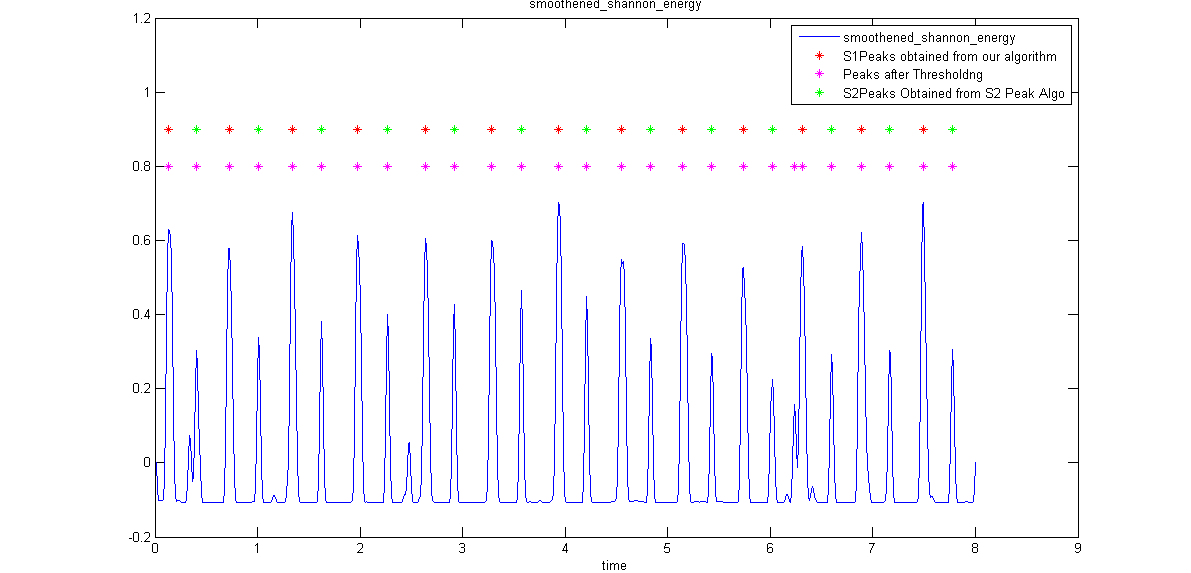
\includegraphics[width=500pt, height=300pt]{ATraining_8_Algo_S2Peaks_step3.png}
\caption{$S_1$ and $S_2$ peaks detected from our algorithm}
\end{center}
\end{figure}


\section{Results for Challenge1: Segmentation}


\begin{figure}
\begin{center}
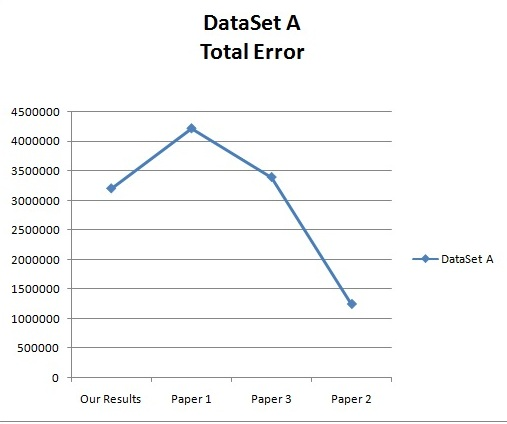
\includegraphics[width=300pt, height=200pt]{TotalError-DataSetA.jpg}
\caption{}
\end{center}
\end{figure}


\begin{center}
\begin{tabular}{|l |c |l |l|}
\hline
File name & Total of Heart beat & Average Error & Total Error \\
\hline
201101070538.aif & 8.5 & 110845.5882 & 3202646.232347 \\
201101151127.aif&5.5&107023.1818& \\
201102081152.aif&9.5&179690& \\
201102201230.aif&10.5&1094.666667& \\
201102270940.aif&1&1349700.5& \\
201103101140.aif&9.5&39444.63158& \\
201103140135.aif&3&599000.3333& \\
201103170121.aif&5&344710.1& \\
201104122156.aif&6.5&155425.2308& \\
201106151236.aif&5&315712& \\
\hline
\end{tabular}
\end{center}
\section{Challenge 2: Classification}
For Classification the first task was to select attributes to base our classifier on. We selected a set of 14 attributes which are described in the subsection . Then we tried classification using three classifiers, we used Decision Trees, SVM with Gaussian kernel and Neural Networks with one hidden layer and hidden neurons.

\subsection{Attribute Selection}
An instance of the data is the .wav file that stores the data for each of the sound files. After this we created attributes for each of the instances depending on the data. These attributes have been described as below:
\begin{enumerate}
\item \textbf{Best frequency}: The value of the time frequency of the heart beat is stored here. The time period of the heart beats is calculated as the average value of the time difference between the $S_1$ peaks. Inverse of the time period gives the heart beat frequency.
\item \textbf{Time Period Variance} : Variance of the time period (i.e the distance between two consecutive $S_1$ peaks) of the heart beats 
\item \textbf{Length of Systolic period}: The average value of the time period between an $S_1$ and an $S_2$ peak is termed the systolic period of the heart beat. 
\item \textbf{Length of Diastolic period} : The average value of time difference between the $S_2$ peak and the $S_1$ peak of the next heart beat is stored as the Diastolic period.
\item \textbf{Diastolic period length variance} : variance of Diastolic period
\item \textbf{Systolic period length variance} : variance of Systolic Period
\item \textbf{Number of peaks after threshold} : Number of peaks obtained after the first step of thresholding
\item \textbf{Number of peaks finally} : The final number of $S_1$ and $S_2$ peaks obtained after all the steps of the algorithm
\item \textbf{$S_1$ Peaks Energy} : For each of the $S_1$ Peak the Shannon energy is calculated in a window of size 22 around it. This is then summed over all the peaks and then divided by the time length of the signal to obtain the normalized $S_1$ Peaks energy
\item \textbf{$S_2$ Peaks Energy} : The energy of the $S_2$ peaks is calculated in the same way as the for $S_1$ peaks
\item \textbf{Extra Peaks Energy} : All the peaks after thresholding that were neither $S_1$ nor $S_2$ are stored as the extra peaks. Energy is calculated over all these peaks and then normalized with respect to the time length of the signal.
\item \textbf{Systolic Period Energy} : The systolic period energy is calculated between the region of $S_1$ and $S_2$ peaks of the same heart beat
\item \textbf{Diastolic Period Energy} : The diastolic period energy is calculated as the energy between $S_2$ peak of one beat and the $S_1$ peak of the next beat
\item \textbf{Ratio of number of peaks after thresholding to the number of peaks after final step} : This is the ratio of the number of peaks found initially after thresholding to final sum of $S_1$ and $S_2$ peaks. We expect this value to be large for the murmur category.

\section{Challenge 2 Results}
The image below shows the result of our classifiers on Dataset A (collected from IPhone App). We show below the comparison of precision for two of our classifiers (Decision Trees and SVM with Gaussian kernel) with the results of the top 2 submissions in the contest. The first two point in the graph show our results. \\

\begin{figure}
\begin{center}
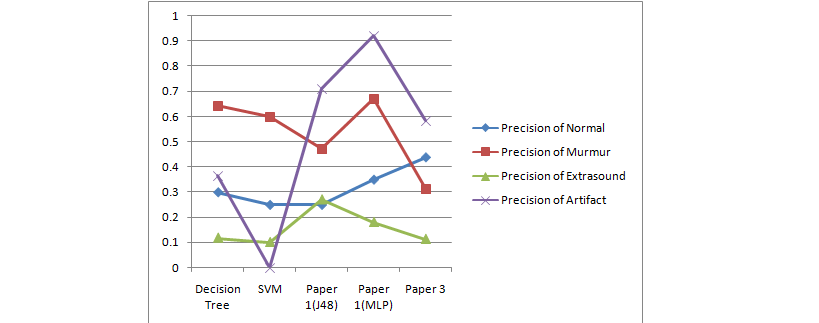
\includegraphics[height=200pt, width=450pt]{Dataseta.png}
\caption{Errors Computed for the test files in dataset A}
\end{center}
\end{figure}

The figure below shows the result of our classifiers on Dataset B, the data collected from clinical trials.\\

\begin{figure}
\begin{center}
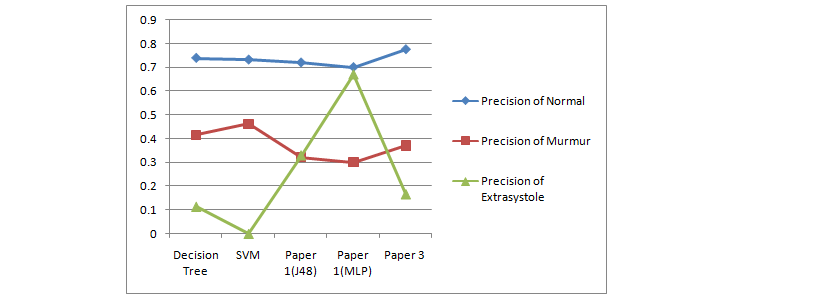
\includegraphics[width= 450pt, height=200pt]{datasetb.png}\\
\caption{Comparison of Precision Scores with other papers on Dataset A}
\end{center}
\end{figure}

In the next figure we compare the overall precision of our results with that of the submissions in the contest.\\

\begin{figure}
\begin{center}
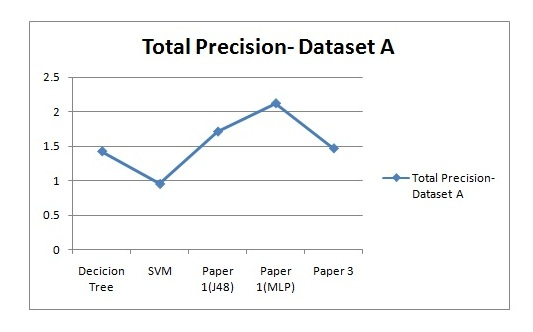
\includegraphics[width=300pt, height=200pt]{TotalPrecicionDatasetA(Challenge2).jpg}\\
\caption{Comparison of Precision Scores with other papers on Dataset B}
\end{center}
\end{figure}


\begin{center}
\begin{tabular}{|c|c|c|c|}
\hline
Filename&Total of Heartbeat&Average Error&Total Error\\ 
\hline
103\_1305031931979\_B.aiff&12&1044.583333&108270.78785686\\ 
103\_1305031931979\_D2.aiff&9&1146.555556&\\ 
106\_1306776721273\_B1.aiff&3.5&2082.714286&\\ 
106\_1306776721273\_C2.aiff&2&5171.75&\\ 
106\_1306776721273\_D1.aiff&3.5&615.57&\\ 
106\_1306776721273\_D2.aiff&6.5&3559&\\ 
107\_1305654946865\_C1.aiff&7&42.85714286&\\ 
126\_1306777102824\_B.aiff&7&10284&\\ 
126\_1306777102824\_C.aiff&5&1414.9&\\ 
133\_1306759619127\_A.aiff&4&1090.5&\\ 
134\_1306428161797\_C2.aiff&2&1343.25&\\ 
137\_1306764999211\_C.aiff&14&4127.928571&\\ 
140\_1306519735121\_B.aiff&9&8459.167&\\ 
146\_1306778707532\_B.aiff&17&1191.735294&\\ 
146\_1306778707532\_D3.aiff&2.5&1195&\\ 
147\_1306523973811\_A.aiff&1.5&18648&\\ 
148\_1306768801551\_D2.aiff&7.5&1138.933333&\\ 
151\_1306779785624\_D.aiff&4&3117.375&\\ 
154\_1306935608852\_B1.aiff&4&1230&\\ 
159\_1307018640315\_B1.aiff&5.5&1396.727273&\\ 
159\_1307018640315\_B2.aiff&2.5&1439.4&\\ 
167\_1307111318050\_A.aiff&5.5&20858&\\ 
167\_1307111318050\_C.aiff&2&680.4&\\ 
172\_1307971284351\_B1.aiff&3&1569.5&\\ 
175\_1307987962616\_B1.aiff&2&1610.75&\\ 
175\_1307987962616\_D.aiff&9.5&6465.157895&\\ 
179\_1307990076841\_B.aiff&16&1230.40625&\\ 
181\_1308052613891\_D.aiff&2.5&1687.4&\\ 
184\_1308073010307\_D.aiff&26&1198.326923&\\ 
190\_1308076920011\_D.aiff&5&3230.9&\\ 


\hline
\end{tabular}
\end{center}
\end{enumerate}

\section{References}
$^{[1]}$ $"$Heart Sound Segmentation Algorithm Based on Heart Sound Envelolgram$"$ .H Liang, S Lukkarinen, I Hartimo .Helsinki University of Technology, Espoo, Finland.\\\\
$^{[2]}$ $"$Sapire DW. Understanding and diagnosing paediatric heart disease:$"$ Heart sounds and murmurs. Norwalk, Connecticut, Applcton \& Langc 1992: 27-43. \\\\
$^{[3]}$ $"$A Robust Heart Sound Segmentation and Classification Algorithm using Wavelet Decomposition and Spectrogram.$"$ Yiqi Deng , Peter J Bentley. Dept. of Computer Science, UCL Malet Place, London. \\\\
$^{[4]}$ $"$Classifying heart sounds using peak location for segmentation and feature construction.$"$ Emanuel Pereira,Elsa Ferreira Gomes. Institute of Engineering (ISEP/IPP) Porto,Portugal. 

\end{document}










